\documentclass[10pt, a4j, dvipdfmx]{jarticle}
\usepackage{titlesec}
\usepackage[dvipdfmx]{graphicx}
\usepackage[dvipdfmx]{color}
\usepackage{float}
\usepackage{wrapfig}
\usepackage{subfigure}
\usepackage{caption}

\graphicspath{{../images/}}

\makeatletter
\newcommand{\figcaption}[1]{\def\@captype{figure}\caption{#1}}
\newcommand{\tblcaption}[1]{\def\@captype{table}\caption{#1}}
\makeatother

\title{トランジスタ増幅}
\author{4年 電子システム工学科 40番  山地 駿徹}


\begin{document}

    \begin{center}
        \LARGE トランジスタの静特性
    \end{center}

    \section*{入力特性の測定方法}
    エミッタ接地回路で,$V_{CE}$を一定に保ち,$V_{BE}$を変化させたときの$I_B$の変化を測定する.
    \begin{figure}[H]
        \begin{minipage}{0.5\hsize}
            \centering
            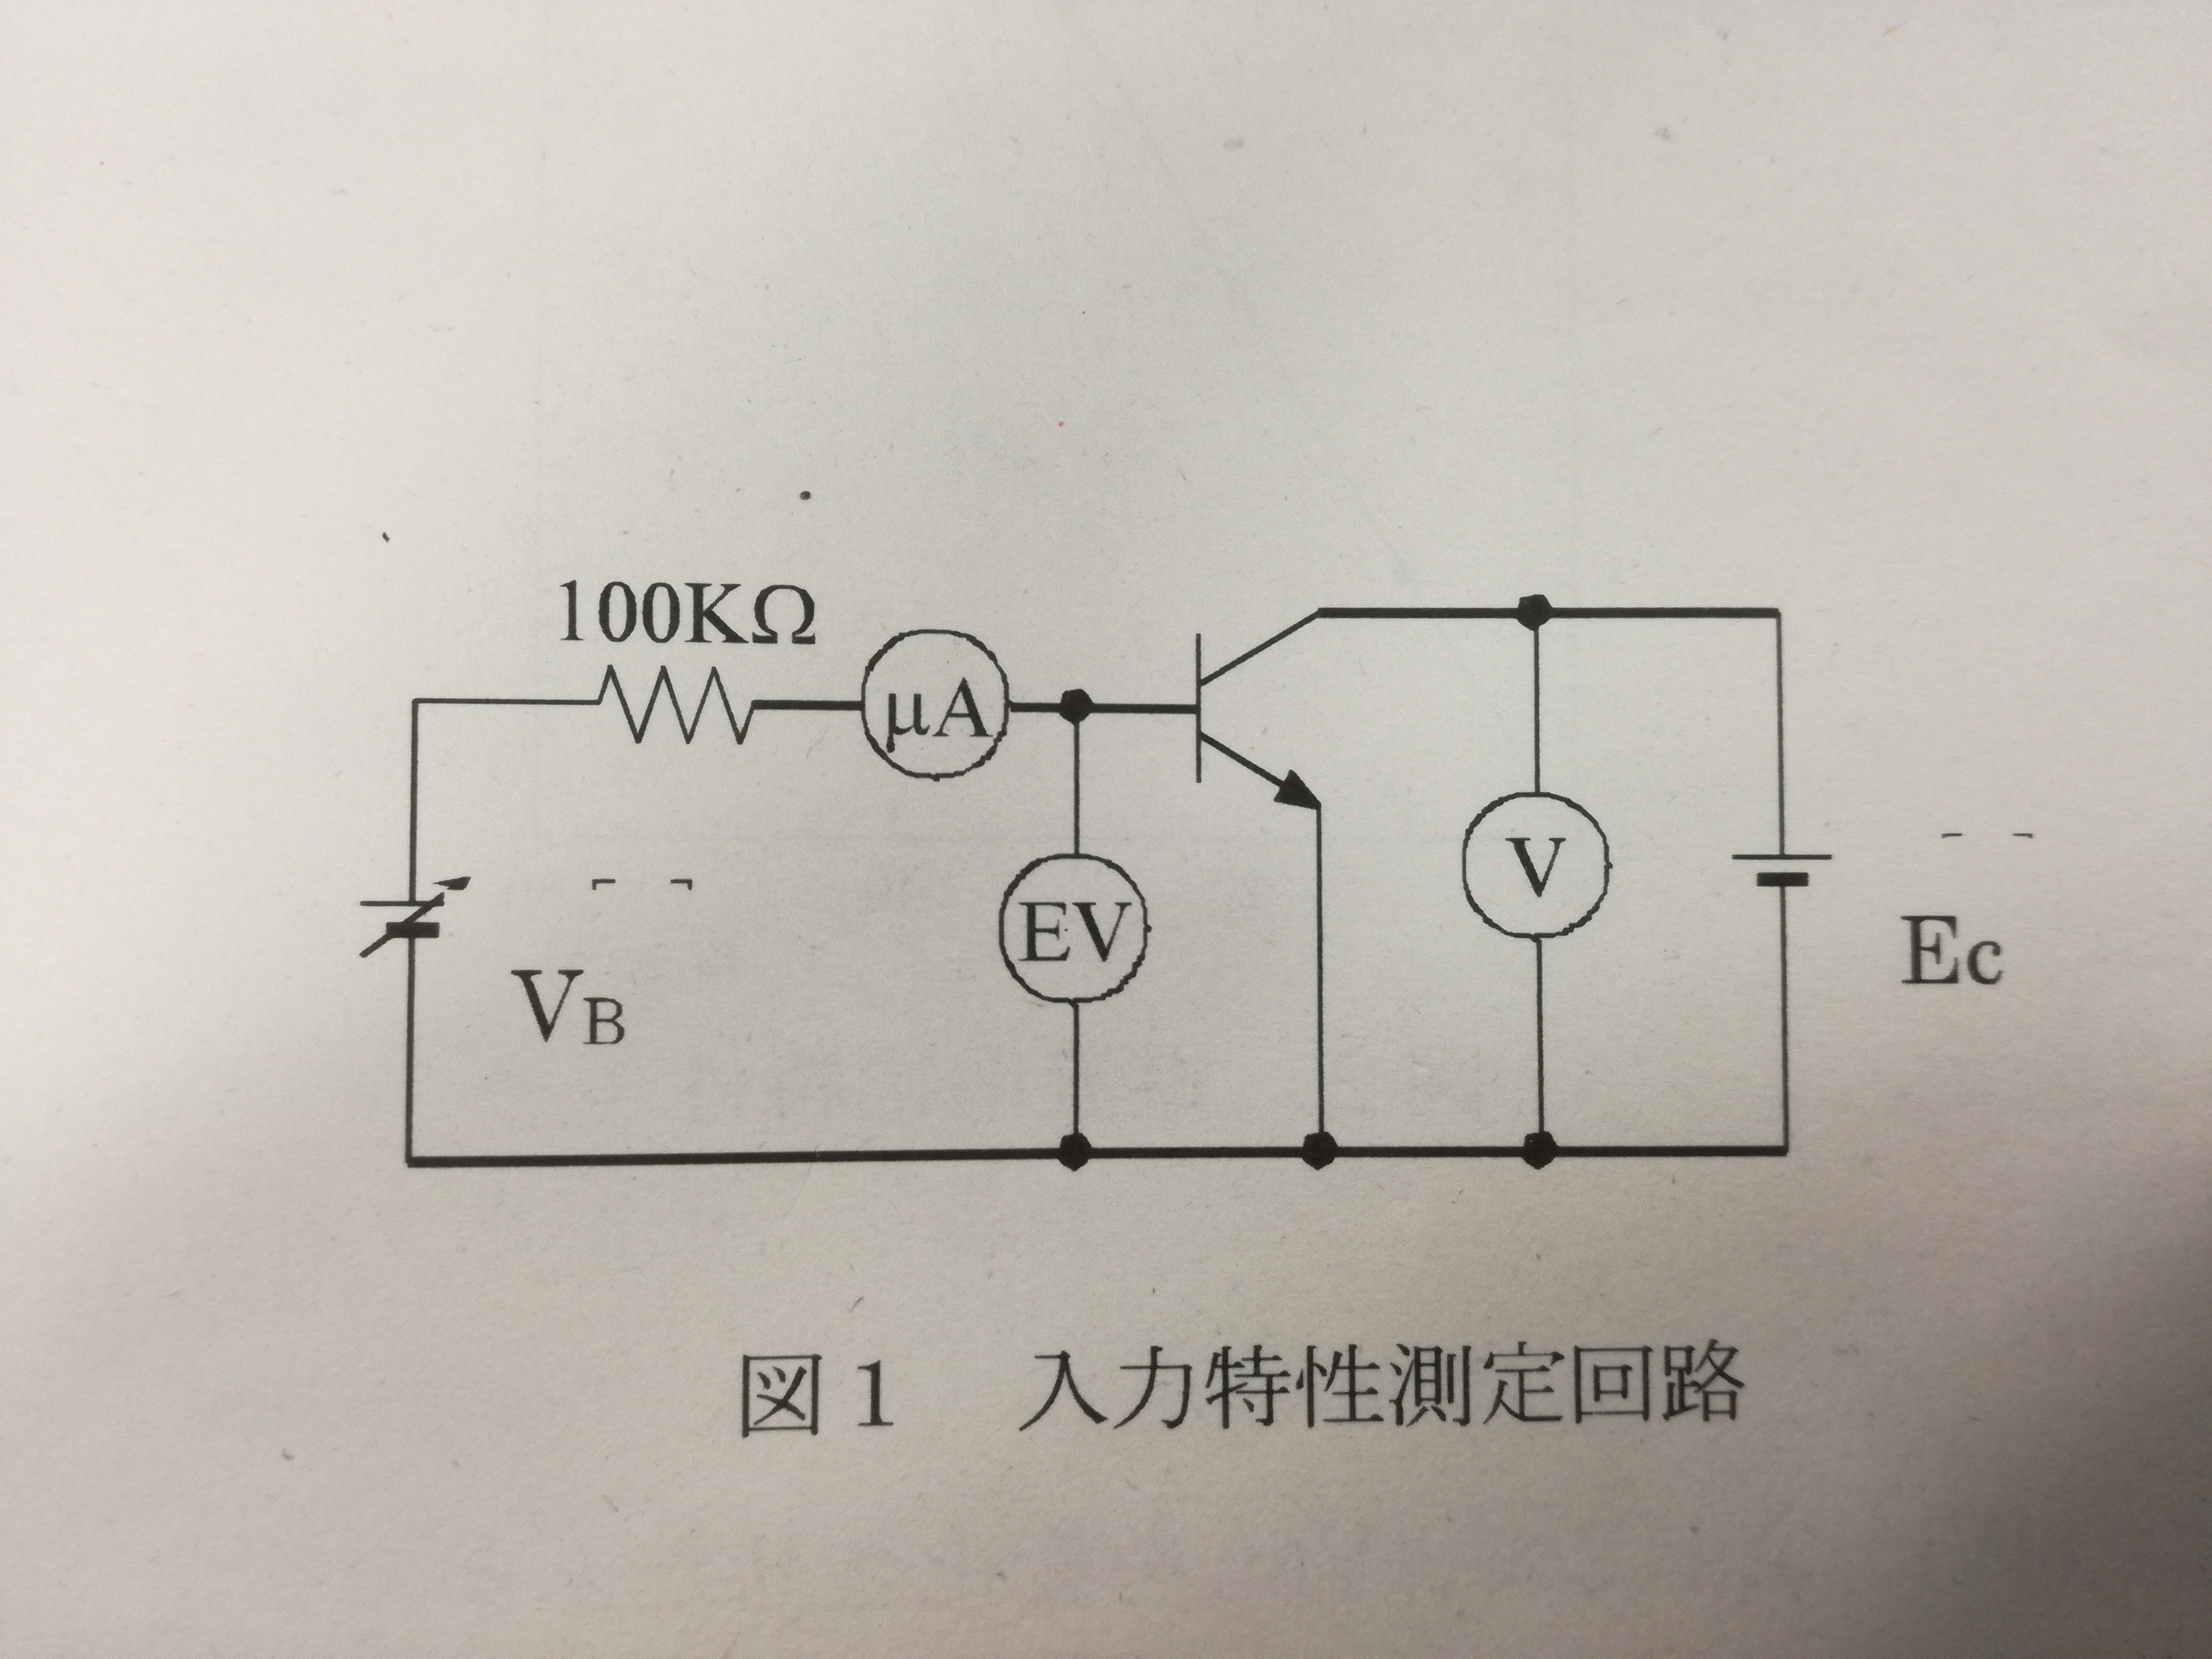
\includegraphics[height=50mm]{fig-1.jpg}
            \caption{入力特性測定回路}
            \label{fig:1}
        \end{minipage}
        \begin{minipage}{0.5\hsize}
            \centering
            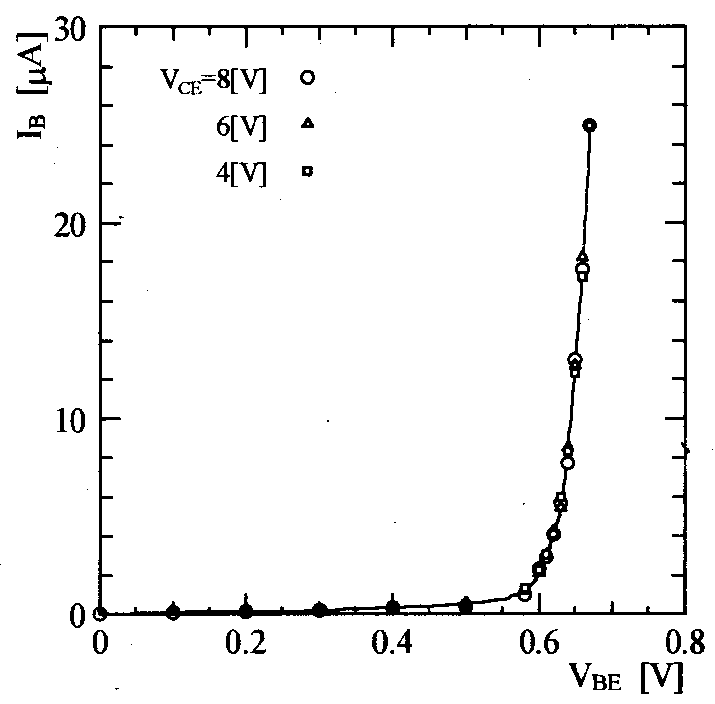
\includegraphics[height=50mm]{fig-2.png}
            \caption{入力特性}
            \label{fig:2}
        \end{minipage}
    \end{figure}

    \section*{出力特性の測定方法}
    エミッタ接地回路で,$I_B$を一定に保ち,$V_{CE}$を変化させたときの$I_C$の変化を測定する.
    \begin{figure}[H]
        \begin{minipage}{0.5\hsize}
            \centering
            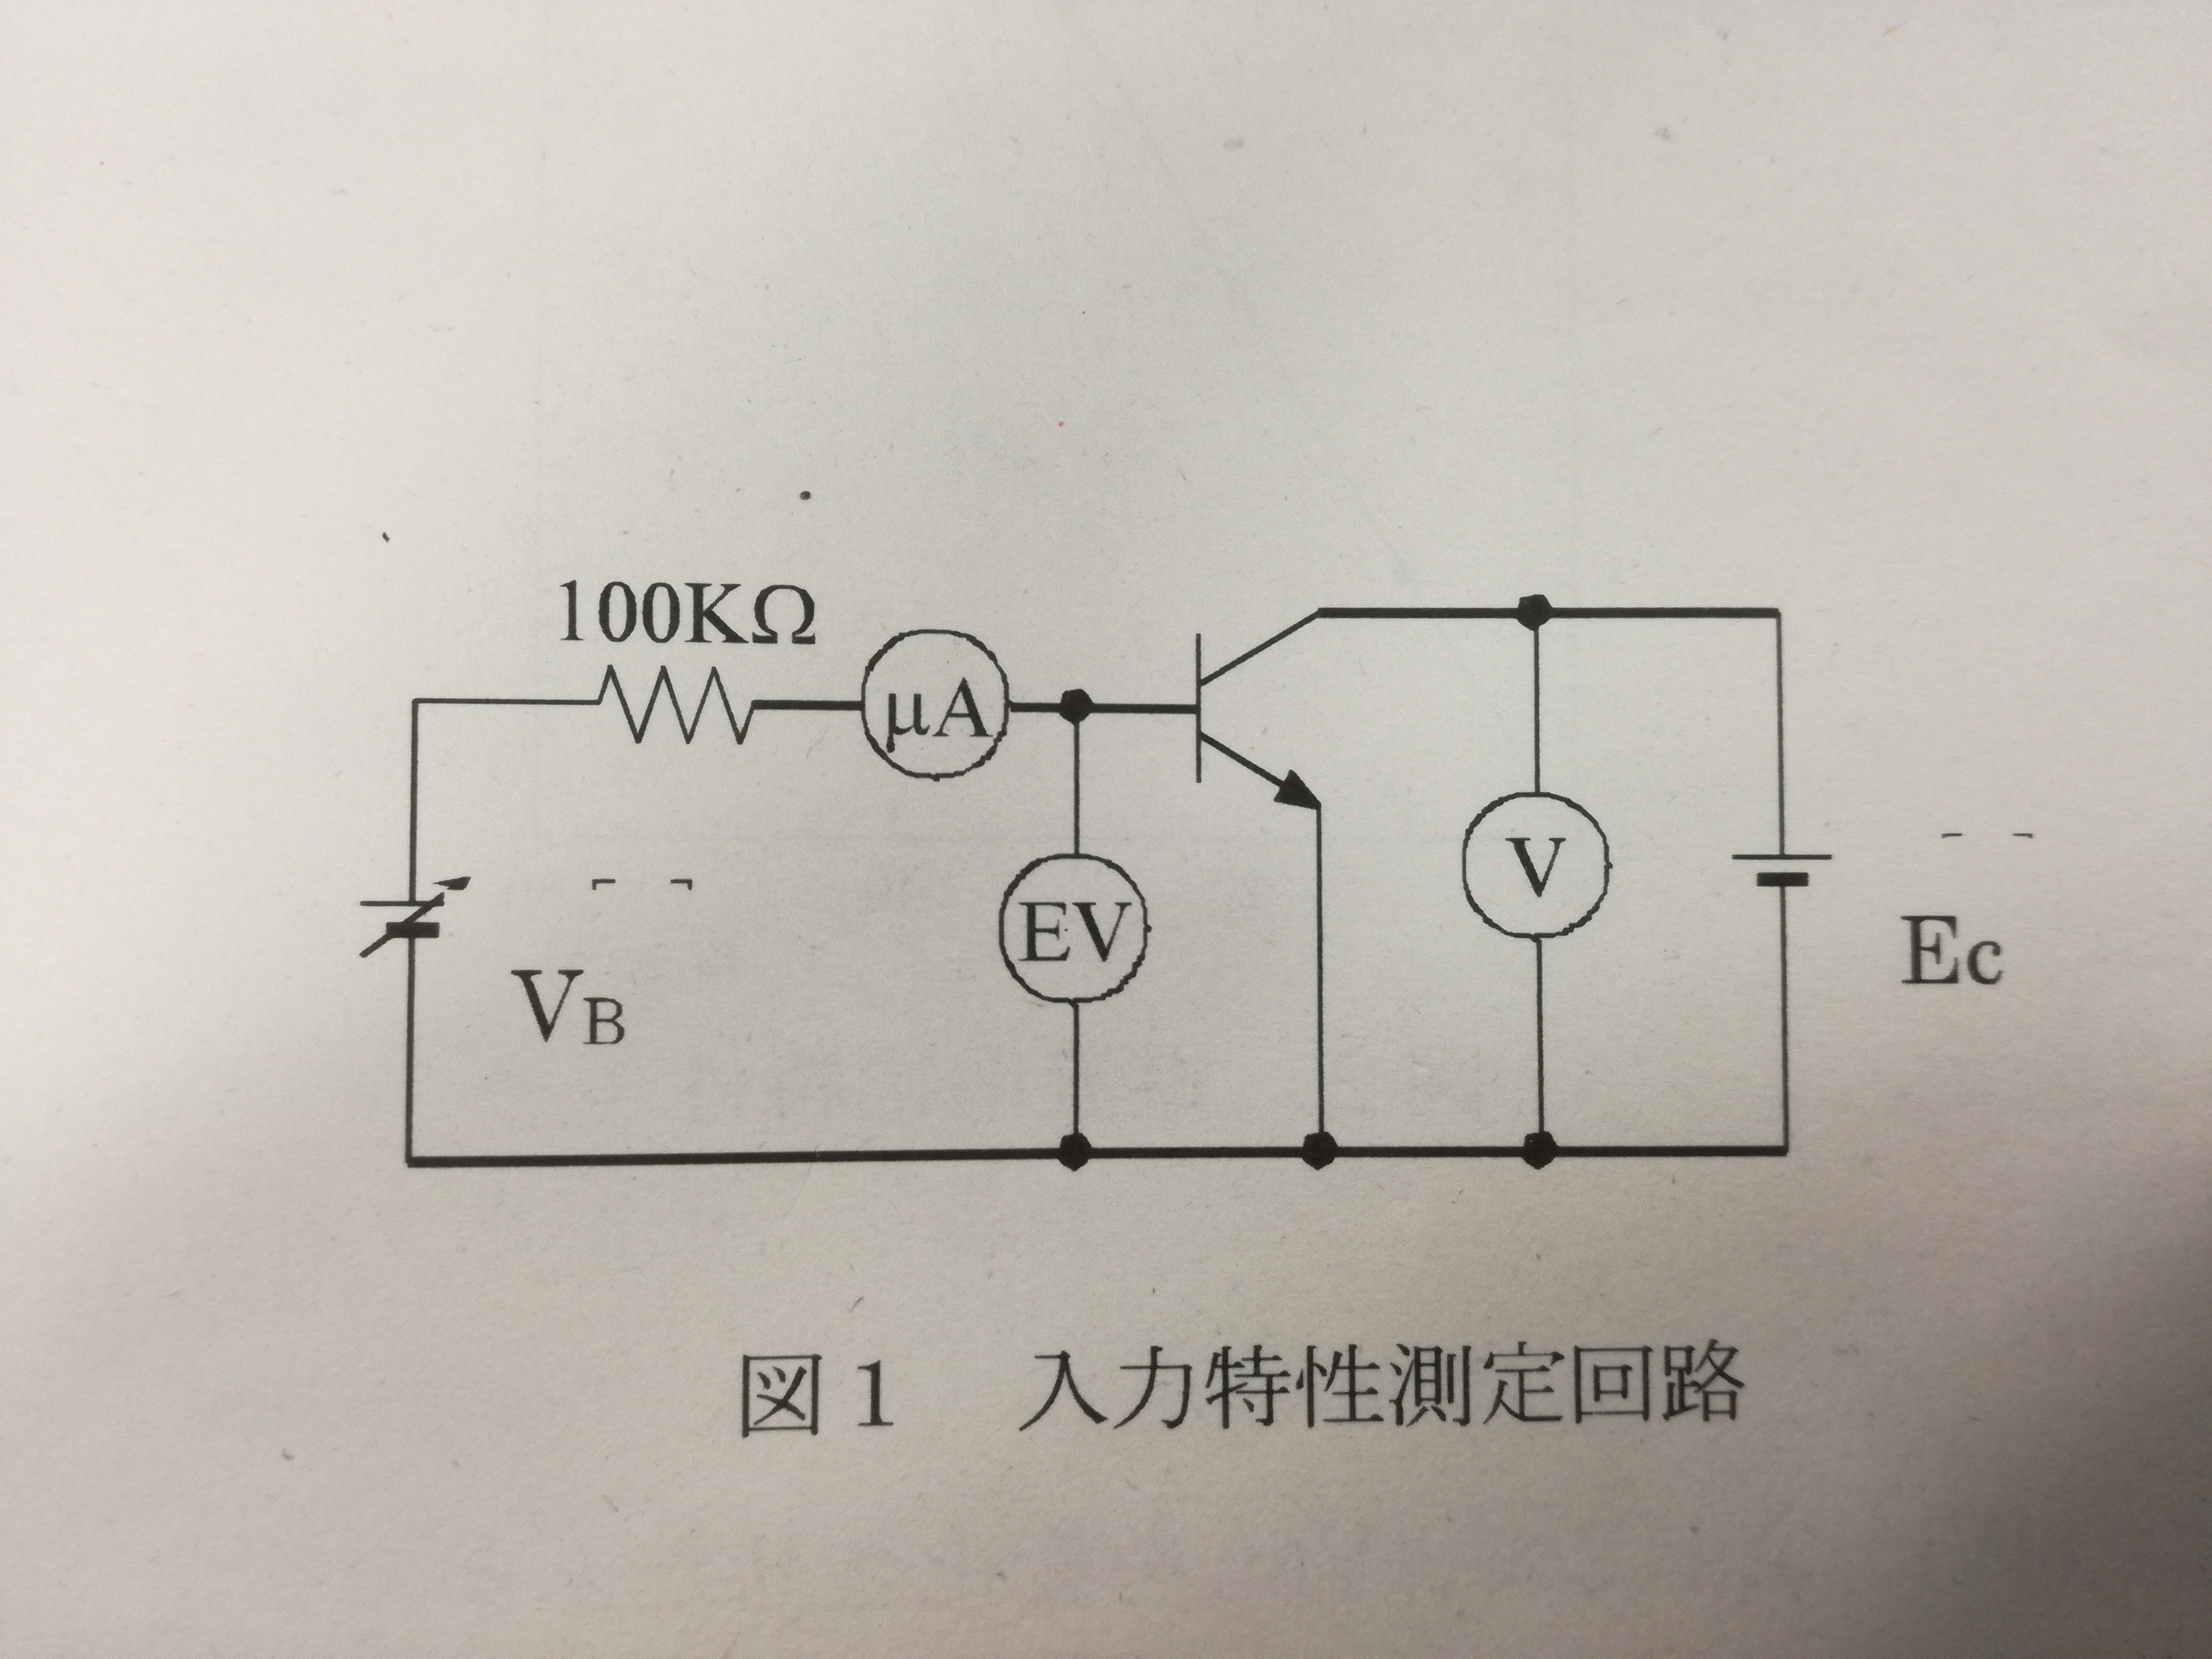
\includegraphics[height=50mm]{fig-1.jpg}
            \caption出力特性測定回路}
            \label{fig:3}
        \end{minipage}
        \begin{minipage}{0.5\hsize}
            \centering
            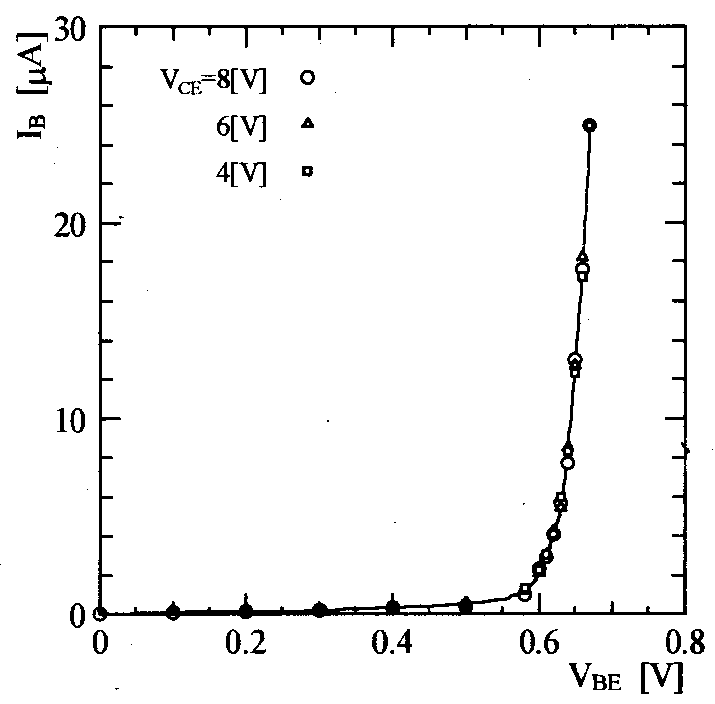
\includegraphics[height=50mm]{fig-2.png}
            \caption{出力特性}
            \label{fig:4}
        \end{minipage}
    \end{figure}
    \section*{吟味事項}
    \begin{enumerate}
        \item 電圧計,電流計の鄧禹給と内部抵抗を調べる.\\電圧計,電流計の接続方法により,計器の内部抵抗による測定誤差について考察する.\\その時の補正方法を考察する.
        \item $V_{CE} = 4[V]$,$I_B = 20[\mu A]$のときの$h$定数を,測定した特性図より求める.
    \end{enumerate}

\end{document}